\documentclass[presentation]{beamer}

\usepackage{tikz}
\usetikzlibrary{positioning,calc}
\usetikzlibrary{shapes.geometric}
\usetikzlibrary{backgrounds}% only to show the bounding box
\usetikzlibrary{shapes,arrows}
\usepackage{pgfplots}
\usepackage{pgfplotstable}
\usetikzlibrary{pgfplots.groupplots}
\pgfplotsset{compat=1.12}
\usepackage{appendixnumberbeamer}
\usepackage{amsmath}
\date{6th July 2016}
\usetheme{metropolis}

\pgfplotscreateplotcyclelist{decent cycle}{%
  {blue, mark=*, mark options={fill=blue},
    mark size=2pt},
  {cyan, mark=square*, mark options={fill=cyan},
    mark size=2pt},
  {magenta, mark=triangle*, mark options={fill=magenta},
    mark size=3pt},
  {blue, mark=*, mark options={fill=blue},
    mark size=2pt},
  {cyan, mark=square*, mark options={fill=cyan},
    mark size=2pt},
  {magenta, mark=triangle*, mark options={fill=magenta},
    mark size=3pt},
}

\pgfplotsset{
  decent/.style={
    cycle list name=decent cycle,
  }
}
\renewcommand{\vec}[1]{\ensuremath{\boldsymbol{#1}}}
\newcommand{\ddt}[1]{\frac{\partial #1}{\partial t}}
\newcommand{\zhat}{\hat{\vec{z}}}
\newcommand{\W}{\ensuremath{\mathbb{W}}}

\DeclareMathOperator{\grad}{grad}
\let\div\relax
\DeclareMathOperator{\div}{div}
\DeclareMathOperator{\curl}{curl}
\newcommand{\vsubset}[1]{\rotatebox[origin=c]{90}{\ensuremath{\subset}}}
\newcommand{\inner}[2]{\ensuremath{\langle #1, #2 \rangle}}
\author{Lawrence Mitchell\inst{1}}
\institute{
\inst{1}Departments of Computing and Mathematics, Imperial College
London
}

\graphicspath{{./\jobname.figures/}}

\newcommand{\arxivlink}[2]{%
  \href{http://www.arxiv.org/abs/#1}%
  {{\small\texttt{arXiv:\,#1\,[#2]}}}%
}
\newcommand{\doilink}[1]{%
  \href{http://dx.doi.org/#1}%
  {{\small\texttt{doi:\,#1}{}}}%
}
\usepackage[url=false,
            doi=true,
            isbn=false,
            style=authoryear,
            firstinits=true,
            uniquename=init,
            backend=biber]{biblatex}

\setbeamertemplate{bibliography item}{}
\renewcommand{\bibfont}{\scriptsize}
\addbibresource{references.bib}

\setlength{\bibitemsep}{1ex}

\renewbibmacro{in:}{}
\DeclareFieldFormat[article]{volume}{\textbf{#1}}
\DeclareFieldFormat{doi}{%
  doi\addcolon%
  {\scriptsize\ifhyperref{\href{http://dx.doi.org/#1}{\nolinkurl{#1}}}
    {\nolinkurl{#1}}}}
\AtEveryBibitem{%
\clearfield{pages}%
\clearfield{issue}%
\clearfield{number}%
}

\usepackage{minted}

\title{Firedrake: automating the finite element method by composing
  abstractions}

\begin{document}
\maketitle

\begin{frame}
  \frametitle{Firedrake team}
  \begin{itemize}
  \item[IC] David A.~Ham, Mikl\'os Homolya, Fabio Luporini, Gheorghe-Teodor
    Bercea, Paul H.~J.~Kelly
  \item[Bath] Andrew T.~T.~McRae
  \item[ECMWF] Florian Rathgeber
  \end{itemize}
  \begin{center}
    \uncover<2->{\url{www.firedrakeproject.org}}\\
    \uncover<3->{\cite{Rathgeber:2015} \arxivlink{1501.01809}{cs.MS}}
  \end{center}
\end{frame}

\section{The right abstraction level}

\begin{frame}[fragile]
  \frametitle{How do \emph{you} solve the Poisson equation?}
  \begin{columns}
    \begin{column}{0.65\textwidth}
\begin{minted}[fontsize=\tiny]{python}
from firedrake import *
mesh = UnitSquareMesh(100, 100)
V = FunctionSpace(mesh, "RT", 2)
Q = FunctionSpace(mesh, "DG", 1)
W = V*Q
u, p = TrialFunctions(W)
v, q = TestFunctions(W)

a = dot(u, v)*dx + div(v)*p*dx + div(u)*q*dx
L = -Constant(1)*v*dx
u = Function(W)
solve(a == L, u, solver_parameters={
    "ksp_type": "gmres", 
    "ksp_rtol": 1e-8,
    "pc_type": "fieldsplit",
    "pc_fieldsplit_type": "schur",
    "pc_fieldsplit_schur_fact_type": "full",
    "pc_fieldsplit_schur_precondition": "selfp",
    "fieldsplit_0_ksp_type": "preonly",
    "fieldsplit_0_pc_type": "ilu",
    "fieldsplit_1_ksp_type": "preonly",
    "fieldsplit_1_pc_type": "hypre"
})
\end{minted}
    \end{column}
    \hspace{-4em}
    \begin{column}{0.5\textwidth}
      Find $u\in V\times Q\subset H(\div)\times L^2$ s.t.
      \begin{align*}
        \inner{u}{v} + \inner{\div v}{p} &= 0 \quad\forall\, v \in V\\
        \inner{\div u}{q} &= -\inner{1}{q}\quad\forall\, q \in Q.
      \end{align*}
    \end{column}
  \end{columns}
\end{frame}


\begin{frame}
  \frametitle{More than a pretty face}

  \begin{block}{Library usability}
    \begin{itemize}
    \item High-level language enables rapid model development
    \item Ease of experimentation
    \item Small model code base
    \end{itemize}
  \end{block}

  \begin{block}{Library development}
    \begin{itemize}
    \item Automation of complex optimisations
    \item Exploit expertise across disciplines
    \item Small library code base
    \end{itemize}
  \end{block}
\end{frame}

\begin{frame}
  \frametitle{Ease of experimentation}
  How much code do you need to change to
  \begin{itemize}
  \item Change preconditioner (e.g.~ILU to AMG)?
  \item Drop terms in the preconditioning operator?
  \item Use a completely different operator to precondition?
  \item Do quasi-Newton with an approximate Jacobian?
  \item Apply operators matrix-free?
  \end{itemize}

  Same ``easy to use'' code must run fast at scale.
\end{frame}

\begin{frame}[standout]
  Can we offer easy experimentation without compromising
  performance?
\end{frame}

\begin{frame}[standout]
  Say \emph{what}, not \emph{how}.
\end{frame}

\begin{frame}
  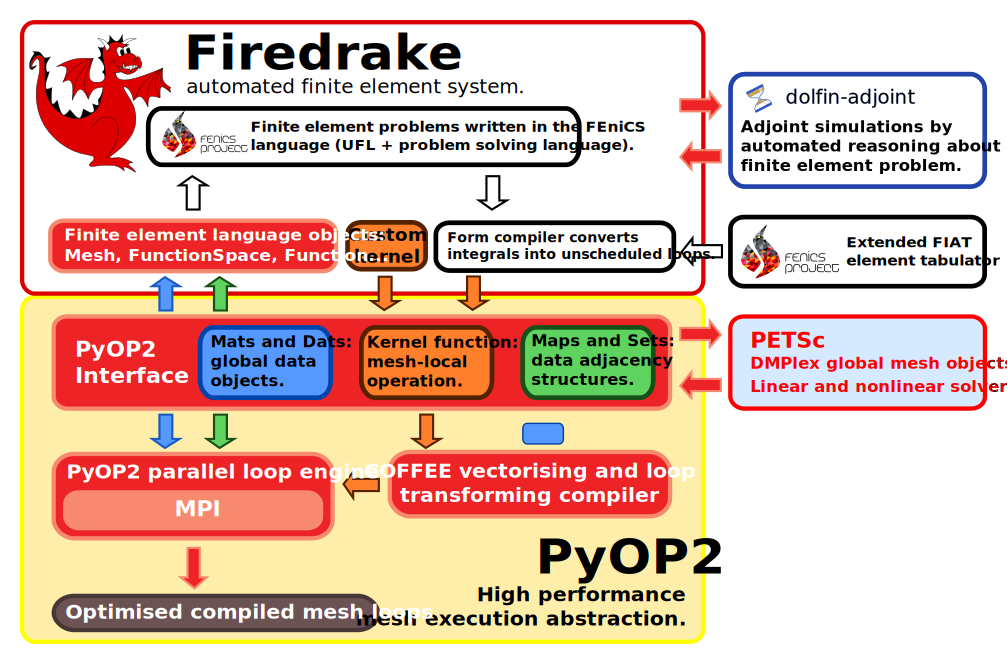
\includegraphics[width=\textwidth]{firedrake-stack}
\end{frame}

\section{Local kernels}

\begin{frame}
  \frametitle{Compiling variational forms}

  We use UFL \parencite{Alnaes:2014} from the FEniCS project for
  specifying variational problems.

  A \emph{form compiler} translates this to low-level executable code
  for evaluating the integral on an element.
\end{frame}

\begin{frame}[fragile]
  \frametitle{An example}
  \begin{columns}
    \begin{column}{0.5\textwidth}
\begin{minted}[fontsize=\tiny]{python}
mesh = UnitTriangleMesh()
V = FunctionSpace(mesh, "CG", 2)
u = TrialFunction(V)
v = TestFunction(V)
a = u*v*dx
\end{minted}
    \end{column}
\hspace{-3em}
    \begin{column}{0.65\textwidth}
\begin{minted}[fontsize=\tiny,mathescape]{c}
void integral(double A[6][6], 
    const double *restrict coords[6])
{
  double t0 = (-1 * coords[0][0]);
  double t1 = (-1 * coords[3][0]);
  /* $t2 \leftarrow |\det J|$ */
  double t2 = fabs(((t0 + (1 * coords[1][0])) *
                     (t1 + (1 * coords[5][0]))) +
                    (-1 * (t0 + (1 * coords[2][0])) *
                     (t1 + (1 * coords[4][0]))));
  static const double t3[6]     = {...};
  static const double t4[6][6]  = {...};
  for (int ip = 0; ip < 6; ip += 1) {
    double t5 = (t3[ip] * t2);
    for (int j = 0; j < 6; j += 1) {
      for (int k = 0; k < 6; k += 1) {
        A[j][k] += t5 * t4[ip][j] * t4[ip][k];
      }
    }
  }
}
\end{minted}
    \end{column}
  \end{columns}
\end{frame}

\begin{frame}[fragile]
  \frametitle{Optimisation of finite element kernels}
  
  \begin{problem}<+->
    Modern optimising compilers do a bad job on finite element
    kernels.
  \end{problem}
  \begin{exampleblock}<+->{Code motion (or not?)}
\begin{minted}[fontsize=\scriptsize]{c}
for (i = 0; i < L; i++ )
   for (j = 0; j < M; j++)
      for (k = 0; k < N; k++)
         A[j][k] += f(i, j)*g(i, k)
\end{minted}
  \end{exampleblock}
  \begin{corollary}<+->
    We need to spoon-feed the compiler already optimised code.
  \end{corollary}
\end{frame}

\begin{frame}
  \frametitle{A job for an expert}
  
  Hardware-aware optimsation of finite element kernels is a job for:
  \begin{itemize}
  \item<2-> A numerical analyst?
  \item<3-> A geodynamicist?
  \item<4-> A computational scientist?
  \item<5-> A computer scientist?
  \end{itemize}
\end{frame}

\begin{frame}
  \frametitle{Automating expertise}
  \begin{itemize}
  \item ``In-person'' case-by-case optimisation \emph{does not scale}
  \item Code generation allows us to package expertise and provide it
    to everyone
  \item Done by a special-purpose kernel compiler
  \end{itemize}
\end{frame}

\begin{frame}[allowframebreaks]
  \frametitle{COFFEE}

  No single optimal schedule for evaluation of every finite element
  kernel.  Variability in
  \begin{itemize}
  \item polynomial degree,
  \item number of fields,
  \item kernel complexity,
  \item working set size,
  \item structure in the basis functions,
  \item structure in the quadrature points,
  \item ...
  \end{itemize}

\pagebreak

\begin{block}{Vectorisation}
  Align and pad data structures, then use intrinsics or rely on
  compiler.\\
  \cite{Luporini:2015} \doilink{10.1145/2687415}
\end{block}

\begin{block}{Flop reduction}
  Exploit \emph{linearity} in test functions to perform factorisation,
  code motion and CSE.  

  \cite{Luporini:2016} \arxivlink{1604.05872}{cs.MS}
\end{block}

\begin{center}
  \url{github.com/coneoproject/COFFEE}
\end{center}
\end{frame}

\section{Global iteration}

\begin{frame}[allowframebreaks]
  \frametitle{Tensions in model development}

  \begin{block}{Performance}
    \begin{itemize}
    \item Keep data in cache as long as possible.  
    \item Manually fuse kernels.
    \item Loop tiling for latency hiding.
    \item ...
    \item Individual components hard to test
    \item Space of optimisations suffers from combinatorial
      explosion.
    \end{itemize}
  \end{block}

\pagebreak
  \begin{block}{Maintainability}
    \begin{itemize}
    \item Keep kernels separate
    \item ``Straight-line'' code
    \item ...
    \item Testable
    \item Even if performance of individual kernels is good, can lose
      \emph{a lot}
    \end{itemize}
  \end{block}

\end{frame}

\begin{frame}[fragile]
  \frametitle{PyOP2}
  A library for expressing data parallel iterations
\begin{description}
\item[{\emph{Sets}}] iterable entities
\item[{\emph{Dats}}] abstract managed arrays (data defined on a set)
\item[{\emph{Maps}}] relationships between elements of sets
\item[{\emph{Kernels}}] local computation
\item[{\emph{par\_loop}}] Data parallel iteration over a set
\end{description}
Arguments to parallel loop indicate how to gather/scatter global
data using \emph{access descriptors}

\begin{minted}[fontsize=\scriptsize]{python}
par_loop(kernel, iterset, data1(map1, READ), data2(map2, WRITE))
\end{minted}
\end{frame}

\begin{frame}
  \frametitle{Key ideas}
  \begin{block}{Local computation}
    Kernels do not know about global data layout.
    \begin{itemize}
    \item Kernel defines contract on local, packed, ordering.
    \item Global-to-local reordering/packing appears in map.
    \end{itemize}
  \end{block}
  \begin{block}{``Implicit'' iteration}
    Application code does not specify explicit iteration order.
    \begin{itemize}
    \item Define data structures, then just ``iterate''
    \item Lazy evaluation
    \end{itemize}
  \end{block}
\end{frame}

\begin{frame}
  \frametitle{Lazy evaluation}
    \begin{itemize}
    \item \verb~par\_loop~ only executed ``when you look at the
      data''.
    \item PyOP2 sees sequence of loops, can reason about them for
      \begin{itemize}
      \item Loop fusion
      \item Loop tiling
      \item Communication coalescing
      \end{itemize}
    \item Application code does not change.  ``What, not how''.
    \end{itemize}
\end{frame}

\section{Did we succeed?}

\begin{frame}
  \frametitle{Experimentation}
  
  With model set up, experimentation is easy

  \begin{itemize}
  \item Change preconditioner: c. 1 line
  \item Drop terms: c. 1-4 lines
  \item Different operator: c. 1-10 lines
  \item quasi-Newton: c. 1-10 lines
  \item Matrix-free: XXX
  \end{itemize}
\end{frame}

\begin{frame}
  \frametitle{Maintainability}
  \begin{columns}
    \begin{column}[t]{0.5\textwidth}
      \begin{block}{Core Firedrake}
        \begin{table}
          \centering
          \begin{tabular}{lc}
            Component & LOC \\
            \hline
            Firedrake & 9000 \\
            PyOP2     & 5000 \\
            TSFC      & 2700 \\
            COFFEE    & 4500 \\
            \hline
            Total     & 21200
          \end{tabular}
        \end{table}
      \end{block}
    \end{column}
    \begin{column}[t]{0.5\textwidth}
      \begin{block}{Shared with FEniCS}
        \begin{table}
          \centering
          \begin{tabular}{lc}
            Component & LOC \\
            \hline
            FIAT & 4000 \\
            UFL     & 13000 \\
            \hline
            Total & 17000
          \end{tabular}
        \end{table}        
      \end{block}
    \end{column}
  \end{columns}
\end{frame}
\begin{frame}[allowframebreaks]
  \frametitle{Performance}

  \begin{block}{Kernel performance}
    \begin{itemize}
    \item COFFEE produces kernels that are better (operation count)
      than existing automated form compilers
    \item Provably optimal in some cases
    \item Good vectorised performance, problem dependent, but up to
      70\% peak for in-cache computation.
    \end{itemize}
  \end{block}

\pagebreak

  \begin{columns}
    \begin{column}{0.7\textwidth}
      \begin{block}{Thetis}
        \begin{itemize}
        \item 3D unstructured coastal ocean model written with
          Firedrake
        \item 5000 LOC, c.~1 person year
        \item Lock exchange test case
          \begin{description}
          \item[Thetis] P1DG-P1DG, triangular wedges.  $24s/s$.
          \item[SLIM] hand-coded/optimised (same numerics),
            $6s/s$
          \end{description}
        \end{itemize}
      \end{block}
    \end{column}
    \begin{column}[t]{0.3\textwidth}
      
\includegraphics[width=2.5cm]{thetis_logo}
    \end{column}
  \end{columns}
  \begin{center}
    \url{github.com/thetisproject/thetis}    
  \end{center}
\end{frame}

\begin{frame}[fragile]
  \frametitle{Abstraction degradation}
  Exposing PyOP2 provides means of writing mesh iterations that are
  not ``assemble a variational form''.

  \begin{exampleblock}{Slope limiters}
    Vertex-based limiters need max/min over incident cells
\begin{minted}[fontsize=\tiny]{python}
par_loop("""
    for (int i=0; i<qmax.dofs; i++) {
        qmax[i][0] = fmax(qmax[i][0], centroids[0][0]);
        qmin[i][0] = fmin(qmin[i][0], centroids[0][0]);
    }
    """,
       dx,
       {'qmax': (max_field, RW),
        'qmin': (min_field, RW),
        'centroids': (centroids, READ)})
\end{minted}
  \end{exampleblock}
\end{frame}

\begin{frame}
  \frametitle{Summary}
  \begin{itemize}
  \item Firedrake provides a layered set of abstractions for finite
    element
  \item Enables automated provision of expertise to model developers
  \item Computational performance is good, often $>50\%$ achievable
    peak.
  \item Hero-coding necessary if you want the last 10-20\%
  \item ...but at what (person) cost?
  \end{itemize}
\end{frame}
\begin{frame}[standout]
  Questions?
\end{frame}

\appendix
\begin{frame}
  \frametitle{References}
  \printbibliography[heading=none]
\end{frame}
\end{document}
